\section{Connecting to a server}
The first part of connecting to a server is knowing the ip address of the server.
Finding the ip address of a server is not a trivial task.
In order for the clients to find a hosted server, that server has to broadcast its address across the whole network.
This can be done by sending packets to a broadcast address and a specified port, as seen in Figure \ref{fig:broadcast}.
The address 255.255.255.255 is the \textit{this network} broadcast address, which means its broadcasts reach clients in the local network.
The server broadcasts its address, the name of the host, and the current amount of players.

\begin{figure}[H]
\centering
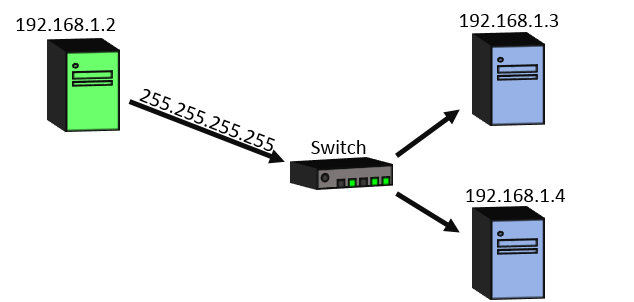
\includegraphics[scale=1]{figures/network/broadcast}
\caption{A server (green) is sending its information packets through the broadcast channel. The switch then forwards the packets to all clients (blue) in the local network.}
\label{fig:broadcast}
\end{figure}

When the client is in the server browser screen, it listens for broadcasts on the same port as the server broadcasts, and will then construct a server list from the data received.
Clicking on one of the servers will then connect the client to that server.